\documentclass[11pt,letterpaper]{report}
\usepackage[margin=0.75in]{geometry}
\usepackage[latin1]{inputenc}
\usepackage{amsmath}
\usepackage{amsfonts}
\usepackage{amssymb}
\usepackage{graphicx}
\usepackage{color}
\graphicspath{{./images/}{IR}}
\usepackage{fancyhdr}
\pagestyle{fancy}
\fancyhead{}
\lhead{CS333}
\chead{Project 3 Report}
\rhead{Andy Keene}
\author{Andy Keene}
\title{Project Three Report\\Introduction to Operating Systems\\ Spring 2017}
\date{}
\begin{document}

\newcommand{\ctrl}[1]{ctrl\,--\,#1}

	\maketitle
	

	\section*{Description}
	For this assignment I learned about improving process management by implementing the xv6 state transition diagram using lists (per state) to increase run-time efficiency of state transitions 
	while maintaining the invariant that each process may be on one and only one list at a time. 
	I also learned about
	adding console ctrl commands, using locks to support atomicity, and about using conditional compilation to both produce two functioning versions of the same operating system and to compile code that demonstrates the list invariant.
		
	\section*{Deliverables}
	The following features were added to xv6:
	
	\begin{itemize}
	
	\item xv6 state lists were added to replace the use of the process array {\tt ptable} and increase efficiency. The lists, and transitions between were modeled after the state transition diagram where each list corresponds to a single process state
	 	(note that the diagram omits the transitions between ZOMBIE, UNUSED and EMBRYO), with the invariant 
		that \emph{each process is on one and only one list at a time}. The lists and their corresponding state are as follows: 
	\begin{figure}[h!]
	\centering
	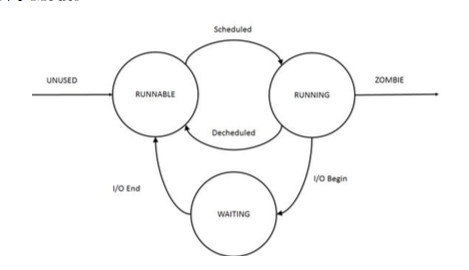
\includegraphics[width=0.3\linewidth]{state-transition.png}
	\caption{State transition diagram}
	\label{fig:0}
	\end{figure}

		\begin{itemize}
			\item Free list. Each process on the free list is the UNUSED state.
			\item Embryo list. Each process on the embryo list is the EMBRYO state.
			\item Ready list. Each process on the ready list is in the RUNNABLE state.
			\item Sleep list. Each process on the sleep list is in the SLEEPING state.
			\item Running list. Each process on the running list is in the RUNNING state.
			\item Zombie List. Each process on the zombie list is in the ZOMBIE state.
		\end{itemize}
		
	\item New console control sequences were added to display information of the corresponding state lists. 
		\begin{itemize}
			\item \ctrl{r} now displays the PID of each processes on the ready list, which corresponds to the processes in the RUNNABLE state. The output displays as: \\
				\\ Ready List Processes: \\ $1 \rightarrow 2 \rightarrow 3 \rightarrow \ldots \rightarrow n$
			\item \ctrl{s} now displays the PID of each processes on the sleep list, which corresponds to the processes in the SLEEPING state. The output displays as: \\
				\\ Sleeping List Processes: \\ $1 \rightarrow 2 \rightarrow 3 \rightarrow \ldots \rightarrow n$
			\item \ctrl{z} now displays the PID and PPID of each processes on the zombie list, which corresponds to the processes in the ZOMBIE state. The output displays as: \\
				\\ Zombie List Processes: \\ $(PID_1, PPID_1) \rightarrow (PID_2, PPID_2) \rightarrow (PID_3, PPID_3) \rightarrow \ldots \rightarrow (PID_n, PPID_n)$
			\item \ctrl{f} now displays the number processes on the free list, which corresponds to the processes in the UNUSED state. The output displays as: \\
				\\ Free List Size: n \\
		\end{itemize}
			
	\end{itemize}
	
\newpage	
	
	% -------- Implementation ---------
	\section*{Implementation}
	
	
	\subsection*{State Lists}
	Note that all changes regarding state lists and their corresponding transitions were done in proc.c, so all line numbers mentioned in regards to these changes refer to the file proc.c. It should also be noted that all changes for this project use the conditional compilation flag {\tt CS333\_P3P4}; often the conditional compilation lines will not included in the line numbers listed for changes.
	To implement the use of state lists in xv6, the following struct to define the state lists was added to proc.c (lines 16-23):
	
\begin{verbatim}
struct StateLists {
  struct proc* ready;
  struct proc* free;
  struct proc* sleep;
  struct proc* zombie;
  struct proc* running;
  struct proc* embryo;
};
\end{verbatim}
	{\tt struct StateLists pLists} was added to the {\tt ptable} struct (line 30) and a {\tt struct proc * next} component was added to the {\tt proc} structure (proc.h line 74) to support linking the processes together in the lists. 
	Next, the following generic helper functions were added to support state transitions between the lists:
		\begin{itemize}
			\item {\tt removeFromStateList(struct proc** stateList, struct proc* p, enum procstate state)} (lines 194-217). Asserts that a lock is held, that p is in the given state, then removes process p from the state list in $O(|statelist|)$ time.
			\item {\tt popHeadFromStateList(struct proc** stateList, struct proc** p, enum procstate state)} (lines 227-242). Asserts that a lock is held, that the head is in the given state, then removes and returns the head of the state list in $O(1)$ time. 
			\item {\tt appendToStateList(struct proc** stateList, struct proc* p, enum procstate state)} (lines 267-287). Asserts that a lock is held, adds the given process p to the end of state list in $O(|statelist|)$ time, then changes it's state to the given state.
			\item {\tt prependToStateList(struct proc** stateList, struct proc* p, enum procstate state)} (lines 293-306). Asserts that the lock is held, then adds the given process p to the head of the state list in $O(1)$ time, and changes its state to the given state.
		\end{itemize}
	
	All state transitions follow the procedure of: obtaining the ptable lock, removing the process from its list through a helper, adding the process to the new list through a helper, then releasing the ptable lock.
	Each call to the aforementioned helper functions passes the process to be added/deleted or returned through, the state list and it's corresponding state (i.e. UNUSED, RUNNABLE, etc.); and all state changes such as {\tt p->state = UNUSED)}
	occur within helper functions that add processes to the list, while the state is asserted to be correct in functions that remove processes. All helper functions accessing a list assert that the lock is held and panic if it is not - this eliminates race conditions 
	within the xv6 state lists and supports atomicity of state transitions which in part helps to ensure our list invariant that is maintained. This invariant is further demonstrated to be held by turning on the {\tt DEBUG} flag which calls {\tt checkProcs} (lines 1155-1175) and {\tt findProc} (lines 1112-1140) before a process is removed, and after a process is added. These functions counts how many lists a process is on and panics if it is not exactly one.
	
	\subsection*{Transitions to Free List}
	The free list is initialized using the existing process table through a call to the helper function {\tt initUnused(void)} (lines 250-261) from {\tt userinit()} (line 400).  After this call, all processes are on the free list. All processes are added to, and removed from the free list using {\tt popFromHead} and {\tt prependToStateList} both of which occur in $O(1)$ complexity - thus the free list is managed in $O(1)$ time. Process are \emph{added} to the 
	free list in the following places:
		\begin{itemize}
			\item If the kernel fails to allocate memory for the process in {\tt allocproc()} it is removed from the embryo list and placed on the free list (lines 361-364). 
			\item If copying a processes into p fails in {\tt fork()} it is removed from the embryo list and placed on the free list (lines 477-478). 
			\item In {\tt wait()} a zombie process may transition from the zombie list and be placed on the free list (lines 673-674).
		\end{itemize}
		
	\subsection*{Transitions to Embryo List}
	Processes are added to the embryo list using {\tt prependToSateList()} and thus occur in $O(1)$ time. Since processes are removed from the free list in $O(1)$ time, transitions from free to embryo occur in $O(1)$ time. 
	Processes are \emph{added} to the embryo list in the following places:
		\begin{itemize}
			\item If {\tt allocproc()} is successful in finding an UNUSED process, it is removed from the free list and added to the embryo list (lines 336, 349).
		\end{itemize}
	
	\subsection*{Ready List}
	To maintain a FIFO scheduling order, processes are \emph{only} added to the end of ready list using {\tt appendToSateList()} and thus occur in $O(n)$ time. Processes are only removed from the head of ready list when the scheduler runs, 
	which removes in $O(1)$. Processes are \emph{added} to the ready list in the following places:
		\begin{itemize}
			\item In {\tt userinit()} initproc is removed from the embryo list and added to the ready list (lines 430-433).
			\item In {\tt fork()} if a process is created it is removed from the embryo list and added to the ready list (lines 508-512).
			\item In {\tt yield()}, which is invoked by the process or through an interrupt, a processes is moved from the running list and added to the ready list (lines 847-848). 
			\item In {\tt wakeup1()} each process sleeping on the channel will be removed from the sleep list and moved to the ready list (lines 946-947)
			\item In {\tt kill()} the process being killed, \emph{if} it is sleeping, will be removed from the sleep list and moved to the ready list (lines 1004-1005).
		\end{itemize}
	
	%\item If {\tt fork()} is successful setting up the process to be used, it is removed from embryo 

	\subsection*{Transitions to Running List}
	Transitions to the running list may only occur within the scheduler, where the scheduler removes the first process on the ready list using {\tt popHeadFromStateList} and adds it to the head of the running list using {\tt prependToStateList}. Since both
	of these list manipulations occur in $O(1)$ time, the transition to the running list occurs in $O(1)$ time. Also, since processes are only added to the end of the running list and removed from the front, a FIFO ordering is maintained.
		\begin{itemize}
			\item If the scheduler is successful in finding a process at the head of the ready list, it is removed and added to the front of the running list (lines 764-765).
		\end{itemize}

	\subsection*{Transitions to Sleep List}
	Processes are added to the sleep list using {\tt prependToSateList()} and thus occur in $O(1)$ time, though they are removed in $O(n)$ time. Processes are added to the sleep list in the following places:
		\begin{itemize}
			\item In {\tt sleep()} the process calling is running so it is removed from the running list and added to the sleep list (lines 902-903).
		\end{itemize}
		
	\subsection*{Transitions to Zombie List}
	Processes are added to the zombie list using {\tt prependToSateList()} and thus occur in $O(1)$ time, though they are removed in $O(n)$ time. Processes are added to the zombie list in the following places:
		\begin{itemize}
			\item In {\tt exit()} the process exiting is running so it is removed from the running list and added to the zombie list (lines 597-598).
		\end{itemize}
		
	\subsection*{Other Process Management Optimizations}
	To optimize process management various dependencies on the process table, {\tt ptable}, were removed. Specifically this occurred in {\tt wait}, {\tt kill}, {\tt wakeup1}, and {\tt exit}.
	
		\begin{itemize}
			\item {\tt wait} (lines 651-693) now uses a method {\tt hasChildren(struct proc * p)} (lines 168-186) to search the embryo, ready, sleep, and running lists for children of the parent - it is called on line 661. {\tt hasChildren} uses 
			{\tt findChild(struct proc* stateList, struct proc* parent)} (lines 150-161) to identify whether a list contains a child of the process. The search is stopped as soon as a child is found. The number of processes
			inspected is reduced by the size of the free list (i.e. $O(NPROC-|free|)$). The zombie list is treated differently since if a child is found it is reaped by removing it from the zombie list and adding it to the free list. 
			
			\item {\tt kill} (lines 990-1011) now uses the helper function {\tt findProcess(struct proc** p, int pid)} (lines 117) to obtain the process with the given PID. {\tt findProcess} just calls {\tt getProcess(struct proc* stateList, struct proc** p, int pid)} (lines 95-110)
			on the embryo, ready, running, sleep, and zombie lists. {\tt kill} obtains the process through the pointer argument and proceeds to handle killing it appropriately. Since {\tt kill} no longer uses the proc table, and instead uses the lists
			its efficiency has increased to $O(NPROC-|free|)$.
			\item {\tt wakeup1} (lines 935-952) now \emph{only} uses the sleep list to search for processes to wake up and transition them from the sleep list to the runnable list. The search is done in-line. This efficiency is now $O(|sleep|)$
			where $O(|sleep|) \leq O(NPROC|)$ (but commonly much, much less).
			\item {\tt exit()} (lines 563-693) now abandons it's children by calling {\tt abandonChildren} (lines 71-88) for the embryo, ready, running, sleep and zombie lists. {\tt abandonChildren(struct proc* stateList, struct proc* parent)} searches 
				through the list given and abandons all the parents (calling process) children, by changing their PPID, to {\tt initproc}. If the child is in the ZOMBIE state, {\tt initproc} is woken. There is a slight efficiency performance
				in this modification as {\tt exit} no longer has to look through the entire process table - the number of processes inspected is now reduced by the size of the free list $NPROC-|free|$.
				
			*$|free|$ in $O(NPROC-|free|)$ refers to the size of free at the point the function obtains the lock, commonly this is a non-zero value. The only places where the process table array is still used, as allowed by the project description,
			is in {\tt userinit()}, {\tt procdump()}, and {\tt getprocs()} - all other references have been replaced with the use of process lists.
		\end{itemize}
	
	\newpage
		
	% ---- console commands ----	
	\subsection*{New Console Commands}
	To support new console commands, changes were made to the files: console.c to trigger the appropriate printing in response to the \ctrl{char} input; defs.h to define the prototype for the kernel side function that prints the appropriate information; 
	and to proc.c to define the function for displaying the list information. All functions such as {\tt dofreelistinfo()} that display list information obtain the ptable lock before traversing the appropriate list and release it upon completion.
		\begin{itemize}
			\item \ctrl{r} 
				\begin{itemize}
					\item Function prototype was added to defs.h (line 124)
					\item In console.c a flag was initialized (line 194), logic for the case of input 'R' was added (lines 219-221), and the logic for triggering the kernel side function to display information was added (lines 250-252)
					\item In proc.c the function {\tt readylistinfo()} was added (lines 1180-1195) to display the PID of each process on the ready list as: \\
						\\ Ready List Processes: \\ $1 \rightarrow 2 \rightarrow 3 \rightarrow \ldots \rightarrow n$
				\end{itemize}
				
			\item \ctrl{s} 
				\begin{itemize}
					\item Function prototype was added to defs.h (line 125)
					\item In console.c a flag was initialized (line 195), logic for the case of input 'S' was added (lines 225-227), and the logic for triggering the kernel side function to display information was added (lines 256-258)
					\item In proc.c the function {\tt sleepinglistinfo()} was added (lines 1217-1233) to display the PID of each process on the sleep list as: \\
						\\ Sleeping List Processes: \\ $1 \rightarrow 2 \rightarrow 3 \rightarrow \ldots \rightarrow n$
				\end{itemize}
			
			\item \ctrl{z} 
				\begin{itemize}
					\item Function prototype was added to defs.h (line 126)
					\item In console.c a flag was initialized (line 195), logic for the case of input 'Z' was added (lines 228-231), and the logic for triggering the kernel side function to display information was added (lines 259-261)
					\item In proc.c the function {\tt zombielistinfo()} was added (lines 1237-1255) to display the PID and PPID of each process on the zombie list as: \\
						\\ Zombie List Processes: \\ $(PID_1, PPID_1) \rightarrow (PID_2, PPID_2) \rightarrow (PID_3, PPID_3) \rightarrow \ldots \rightarrow (PID_n, PPID_n)$
				\end{itemize}
			\item \ctrl{f} 
				\begin{itemize}
					\item Function prototype was added to defs.h (line 123)
					\item In console.c a flag was initialized (line 194), logic for the case of input 'F' was added (lines 222-224), and the logic for triggering the kernel side function to display information was added (lines 251-255)
					\item In proc.c the function {\tt freelistinfo()} was added (lines 1200-1213) to display the number of process on the free list as: \\
						\\ Free List Size: n \\
				\end{itemize}
		\end{itemize}
			
	
	
	% -------- Testing --------
	
	\section*{Testing}
	
	\subsection*{Required Tests}
	For reference the required tests are outlined below.
 	\begin{enumerate}
		\item Demonstrate that the free list is correctly initialized when xv6 is booted. Note that {\tt init} and {\tt sh} should be the only two active processes immediately after boot while the rest are unused. Recall that the {\tt NPROC} variable represents the maximum number of processes in xv6.
	
		\item Demonstrate that the free list is correctly updated when a new process is allocated (state transitions from {\tt UNUSED}) and when a process is deallocated (state transitions to {\tt UNUSED}).
	
		\item Demonstrate the {\tt kill} shell command causes a process to correctly transition to the {\tt ZOMBIE}  and then {\tt UNUSED} states. 
	
		\item Demonstrate that round-robin scheduling is enforced. Specifically, the processes that are  already in the ready list are scheduled before processes added afterwards; any process transitioning to the {\tt RUNNING} state are removed from the front of the ready list. Processes transitioning to the {\tt RUNNABLE} state must be added at the back of the ready list.
	
		\item Demonstrate that the sleep list is correctly updated when a process sleeps (state transitions to  {\tt SLEEPING})  and when processes are woken (state transitions from {\tt SLEEPING}).
	
		\item Demonstrate that the zombie list is correctly updated when a process exits (state transitions to {\tt ZOMBIE}) and when a process is reaped (state transitions from  {\tt ZOMBIE}).
	
		\item Demonstrate that output for the console commands \ctrl{r}, \ctrl{f}, \ctrl{s} and \ctrl{z} is correct (7.a, 7.b, 7.c, and 7.d respectively).
	\end{enumerate}
	
	\subsection*{Free, \ctrl{f} and Zombie, \ctrl{z}  (Requirements 1, 2, 6, 7.b, 7.d)}
	This test will demonstrate: that the free list is correctly updated when a process is allocated (transitions from UNUSED) and when a process is deallocated  (transitions to UNUSED); and that the Zombie list is updated correctly when a process exits (transitions from RUNNING to ZOMBIE) and when a process is reaped (transitions from ZOMBIE to UNUSED). \ctrl{f} and \ctrl{z} will also be shown to be correct. The function, {\tt free\_zombie\_tests} will be added in the user program {\tt test} (test.c lines 107-169).
	
	\begin{itemize}
		\item The user program {\tt test} will pause at start, allowing us to press \ctrl{r}, \ctrl{z} and \ctrl{p} to establish a baseline for the state lists at the start of xv6. Since the {\tt \#DEBUG} flag is set while testing, \ctrl{p} will display 
		the value of NPROC, which represents the maximum number of processes available in the system (added to proc.c lines 1048-1050). We expect that since NPROC represents the number of available processes, and \ctrl{p} will display all 
		processes \emph{not} on the UNUSED list by virtue of the code, call these \emph{active processes}, we know that the number of UNUSED processes will be $|NPROCS| - active\  processes$. 
		Thus, we expect the output of \ctrl{f} to match this number.
		
		\item Next, {\tt test} will fork children and save their PIDs until {\tt fork()} returns -1 signifying a process allocation failed. {\tt test} will then sleep, allowing us to press \ctrl{f} \ctrl{p} and \ctrl{z}. Note, all children will spin-run. 
		Since {\tt fork()} may fail when there are no more processes on the UNUSED list to allocate, we expect the UNUSED list to be empty. We expect \ctrl{f} will now display there are 0 processes on the UNUSED list, 
		\ctrl{z} will display nothing since all children are spinning and not exiting, and \ctrl{p} will now show an \emph{additional} number of active processes (in the running or runnable state) equal to that of the initial \ctrl{f} output. 
		The total number of processes shown by \ctrl{p} should be equal to the value of NPROC, and the parent should display a number of children equal to one less than the initial number of free processes (it had to be created itself!). 
		This demonstrates that process allocation, from UNUSED occurs correctly, that the free list was correctly initialized, and that the output of \ctrl{f} is correct.  
				
		\item The parent process {\tt test} will now, in reverse order of creation, kill then reap a child process. We will be notified before, and after, allowing us to press \ctrl{f} and \ctrl{z} at each step. 
		Before any process is killed, we expect the Zombie list to be empty and the Free List output size to be that of its last output. (initially this should be 0). Since {\tt kill()} sends a process to the 
		Zombie state (if it is not already there), when we press \ctrl{z} and \ctrl{f} after a process is killed, but before it's reaped, we expect \ctrl{z} to contain \emph{only} the process killed and \ctrl{f} to not have changed, 
		where the PID of the ZOMBIE process matched the PID of the child being killed, and its PPID matches the parent. After the process is reaped we expect the Zombie list to again be empty and the free list to have 
		increased by 1. With comparison to \ctrl{p} this demonstrates the that transitions to and from the ZOMBIE state are correct, that transitions to the UNUSED state are correct. 
		
		\item We will continue this process until the reaping completes. After all children processes have been reaped and the parent exits we expect that \ctrl{p} will match its original process listing, 
		that \ctrl{f} will display it's initial value, and that \ctrl{z} will be empty! Output from \ctrl{z} and \ctrl{f} in matching semantic output from \ctrl{p} in all stages demonstrate their correctness, thus 
		showing requirements 7.b and 7.d are met.
		
		\end{itemize}
	
\pagebreak	

\begin{figure}[h]
\centering
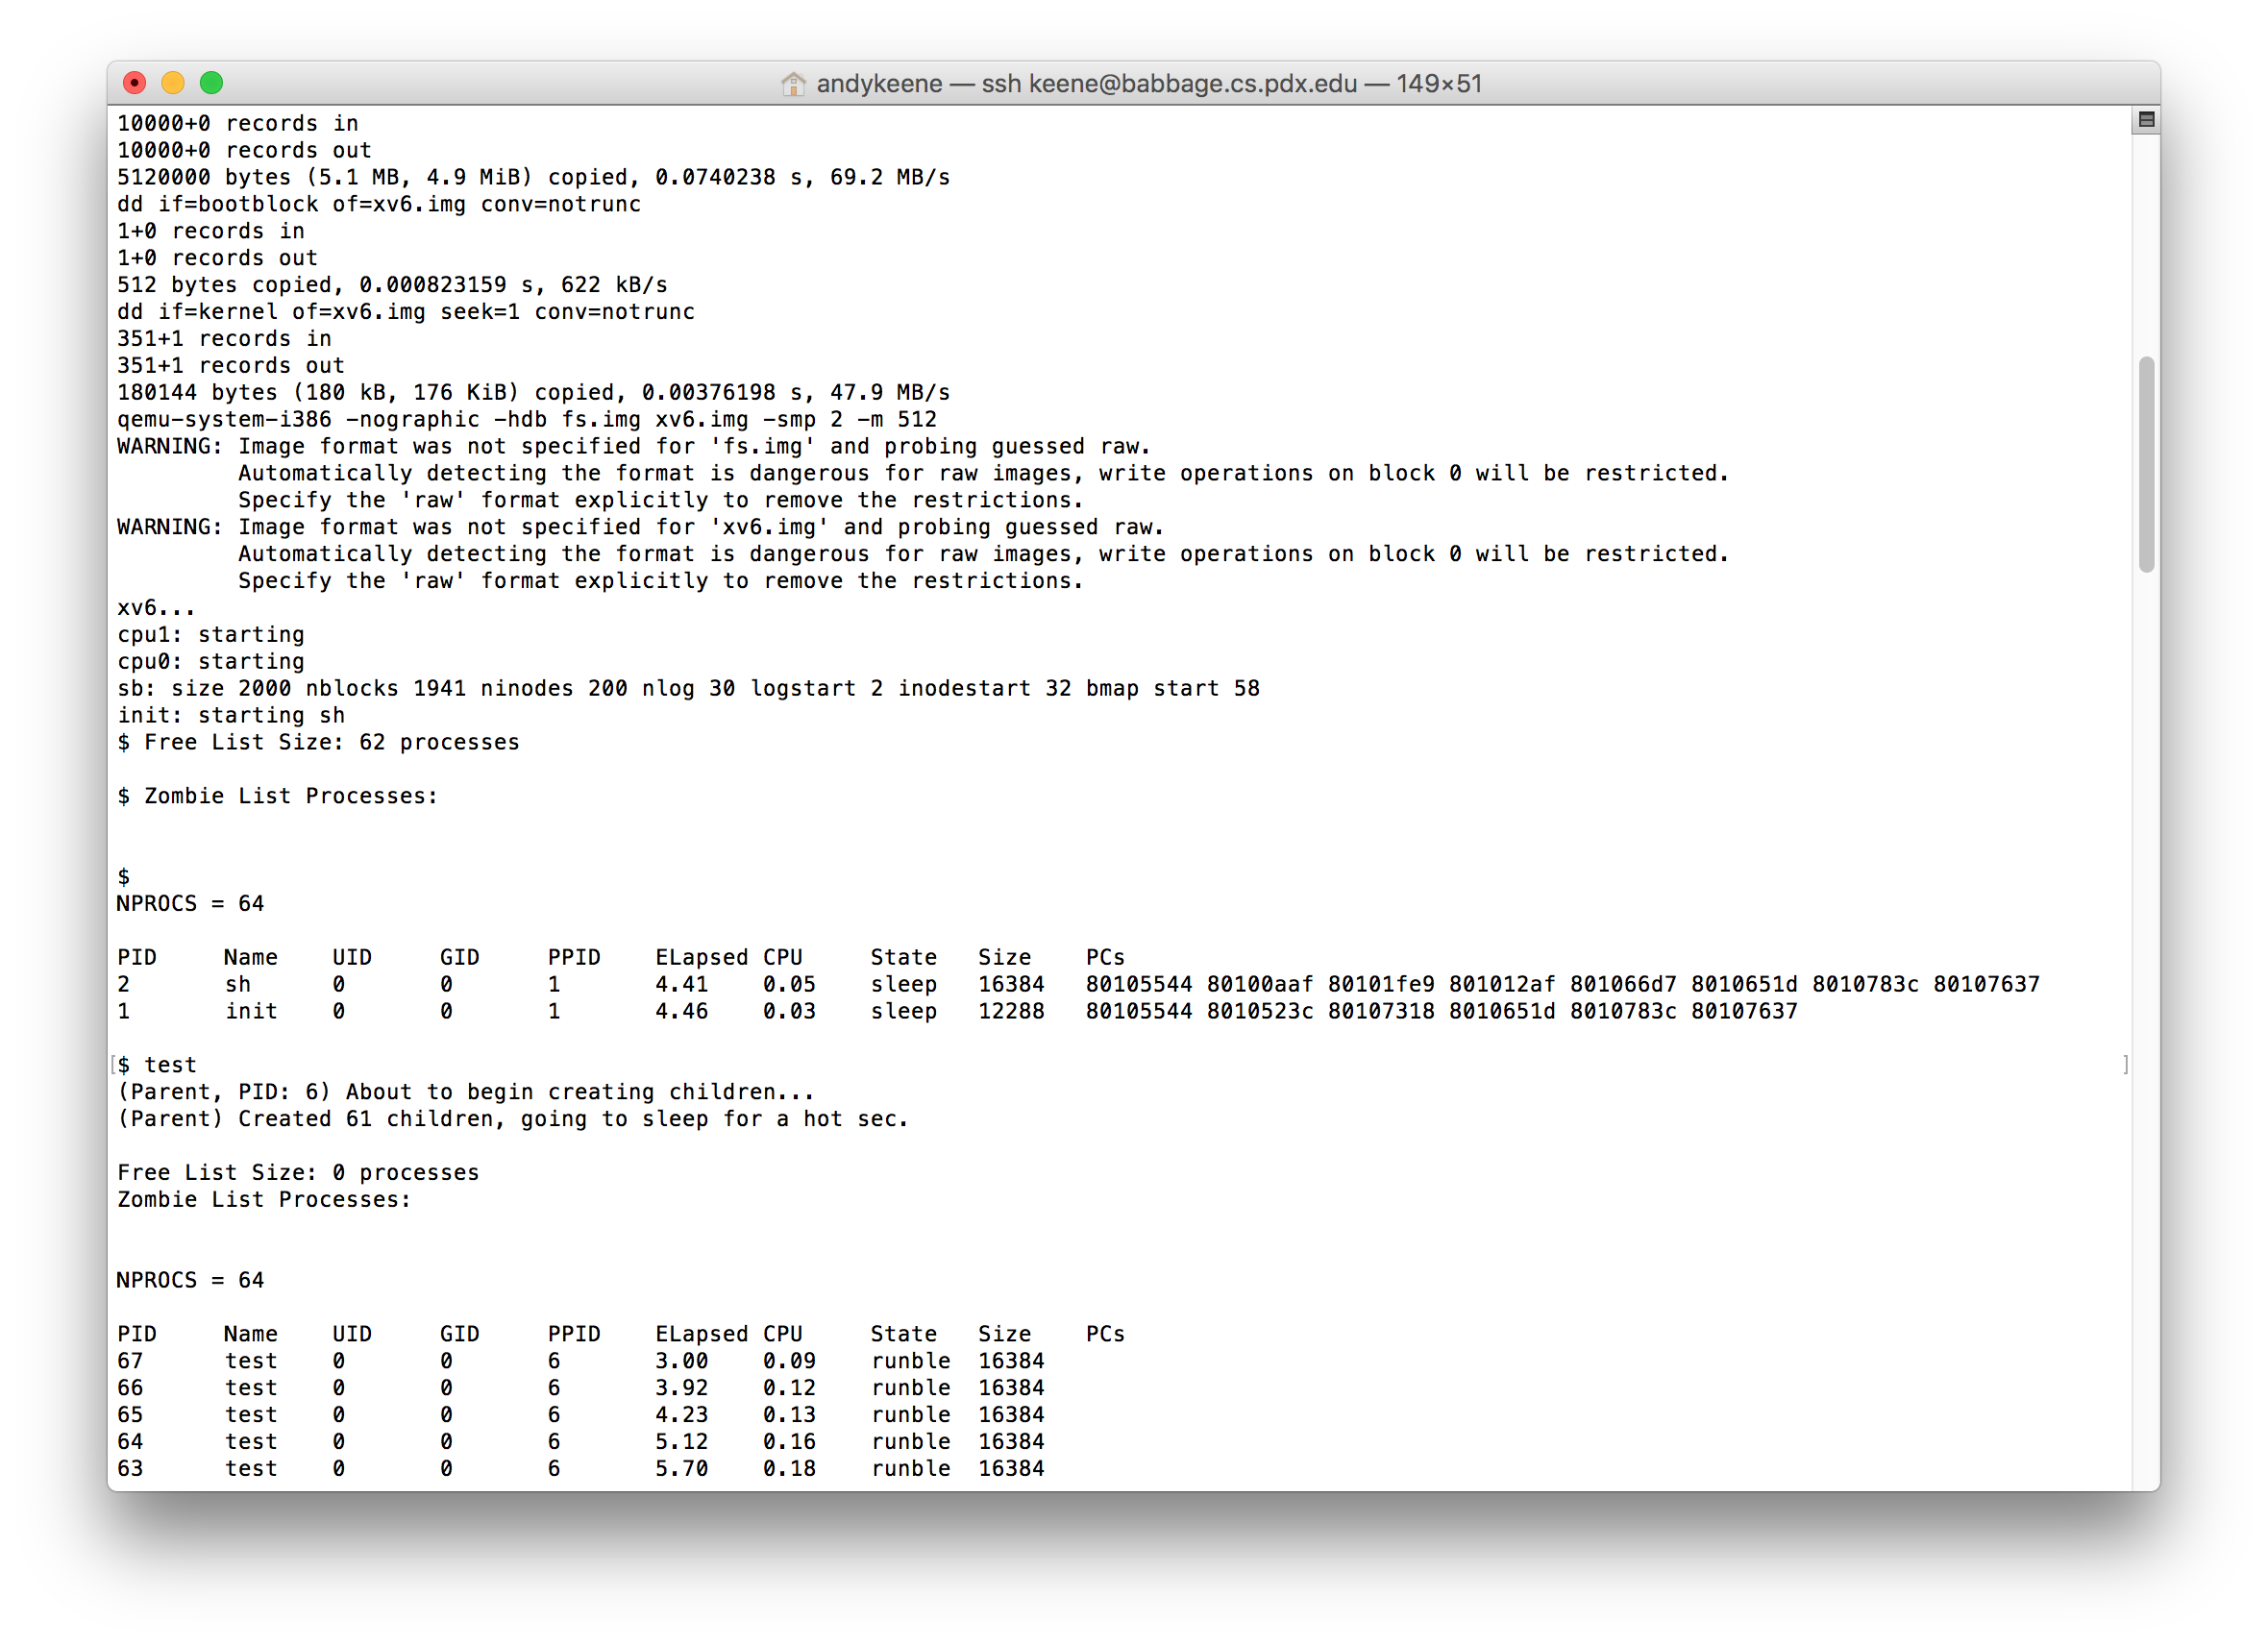
\includegraphics[width=0.8\linewidth]{zombie-init.png}
\caption{Initial list output and after forking}
\label{fig:1}
\end{figure}	

Here we see that \ctrl{p} displays the two processes, {\tt init} and  {\tt sh} along with the value of NPROC being 64. Since NPROC is 64 and there are 2 \emph{active processes}, based on our expectations the output from the free list should be $64-2=62$. The free list output matches this. Additionally, \ctrl{z} is empty which matches \ctrl{p} at this point. This meets our expectations for this stage of the test, thus this step \textbf{PASSES}.


\begin{figure}[h!]
\centering
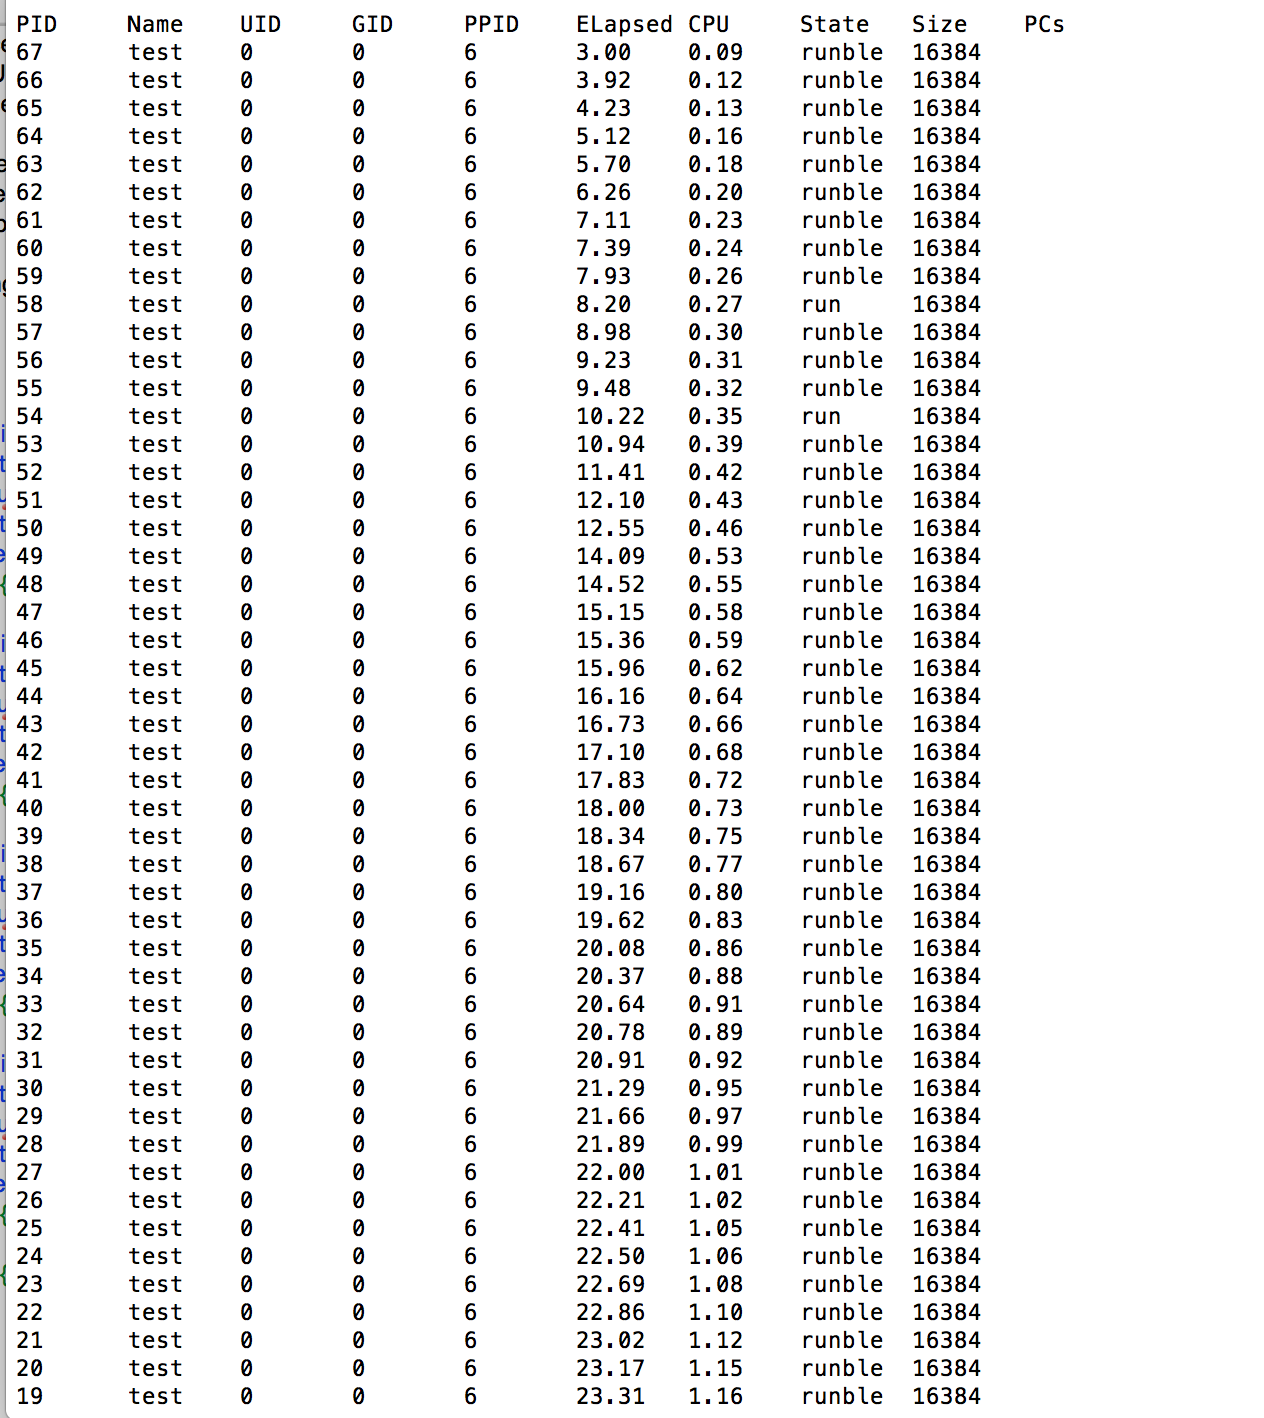
\includegraphics[width=0.8\linewidth]{zombie-allprocs.png}
\caption{ctrl-p output after forking}
\label{fig:2}
\end{figure}

\begin{figure}[h!]
\centering
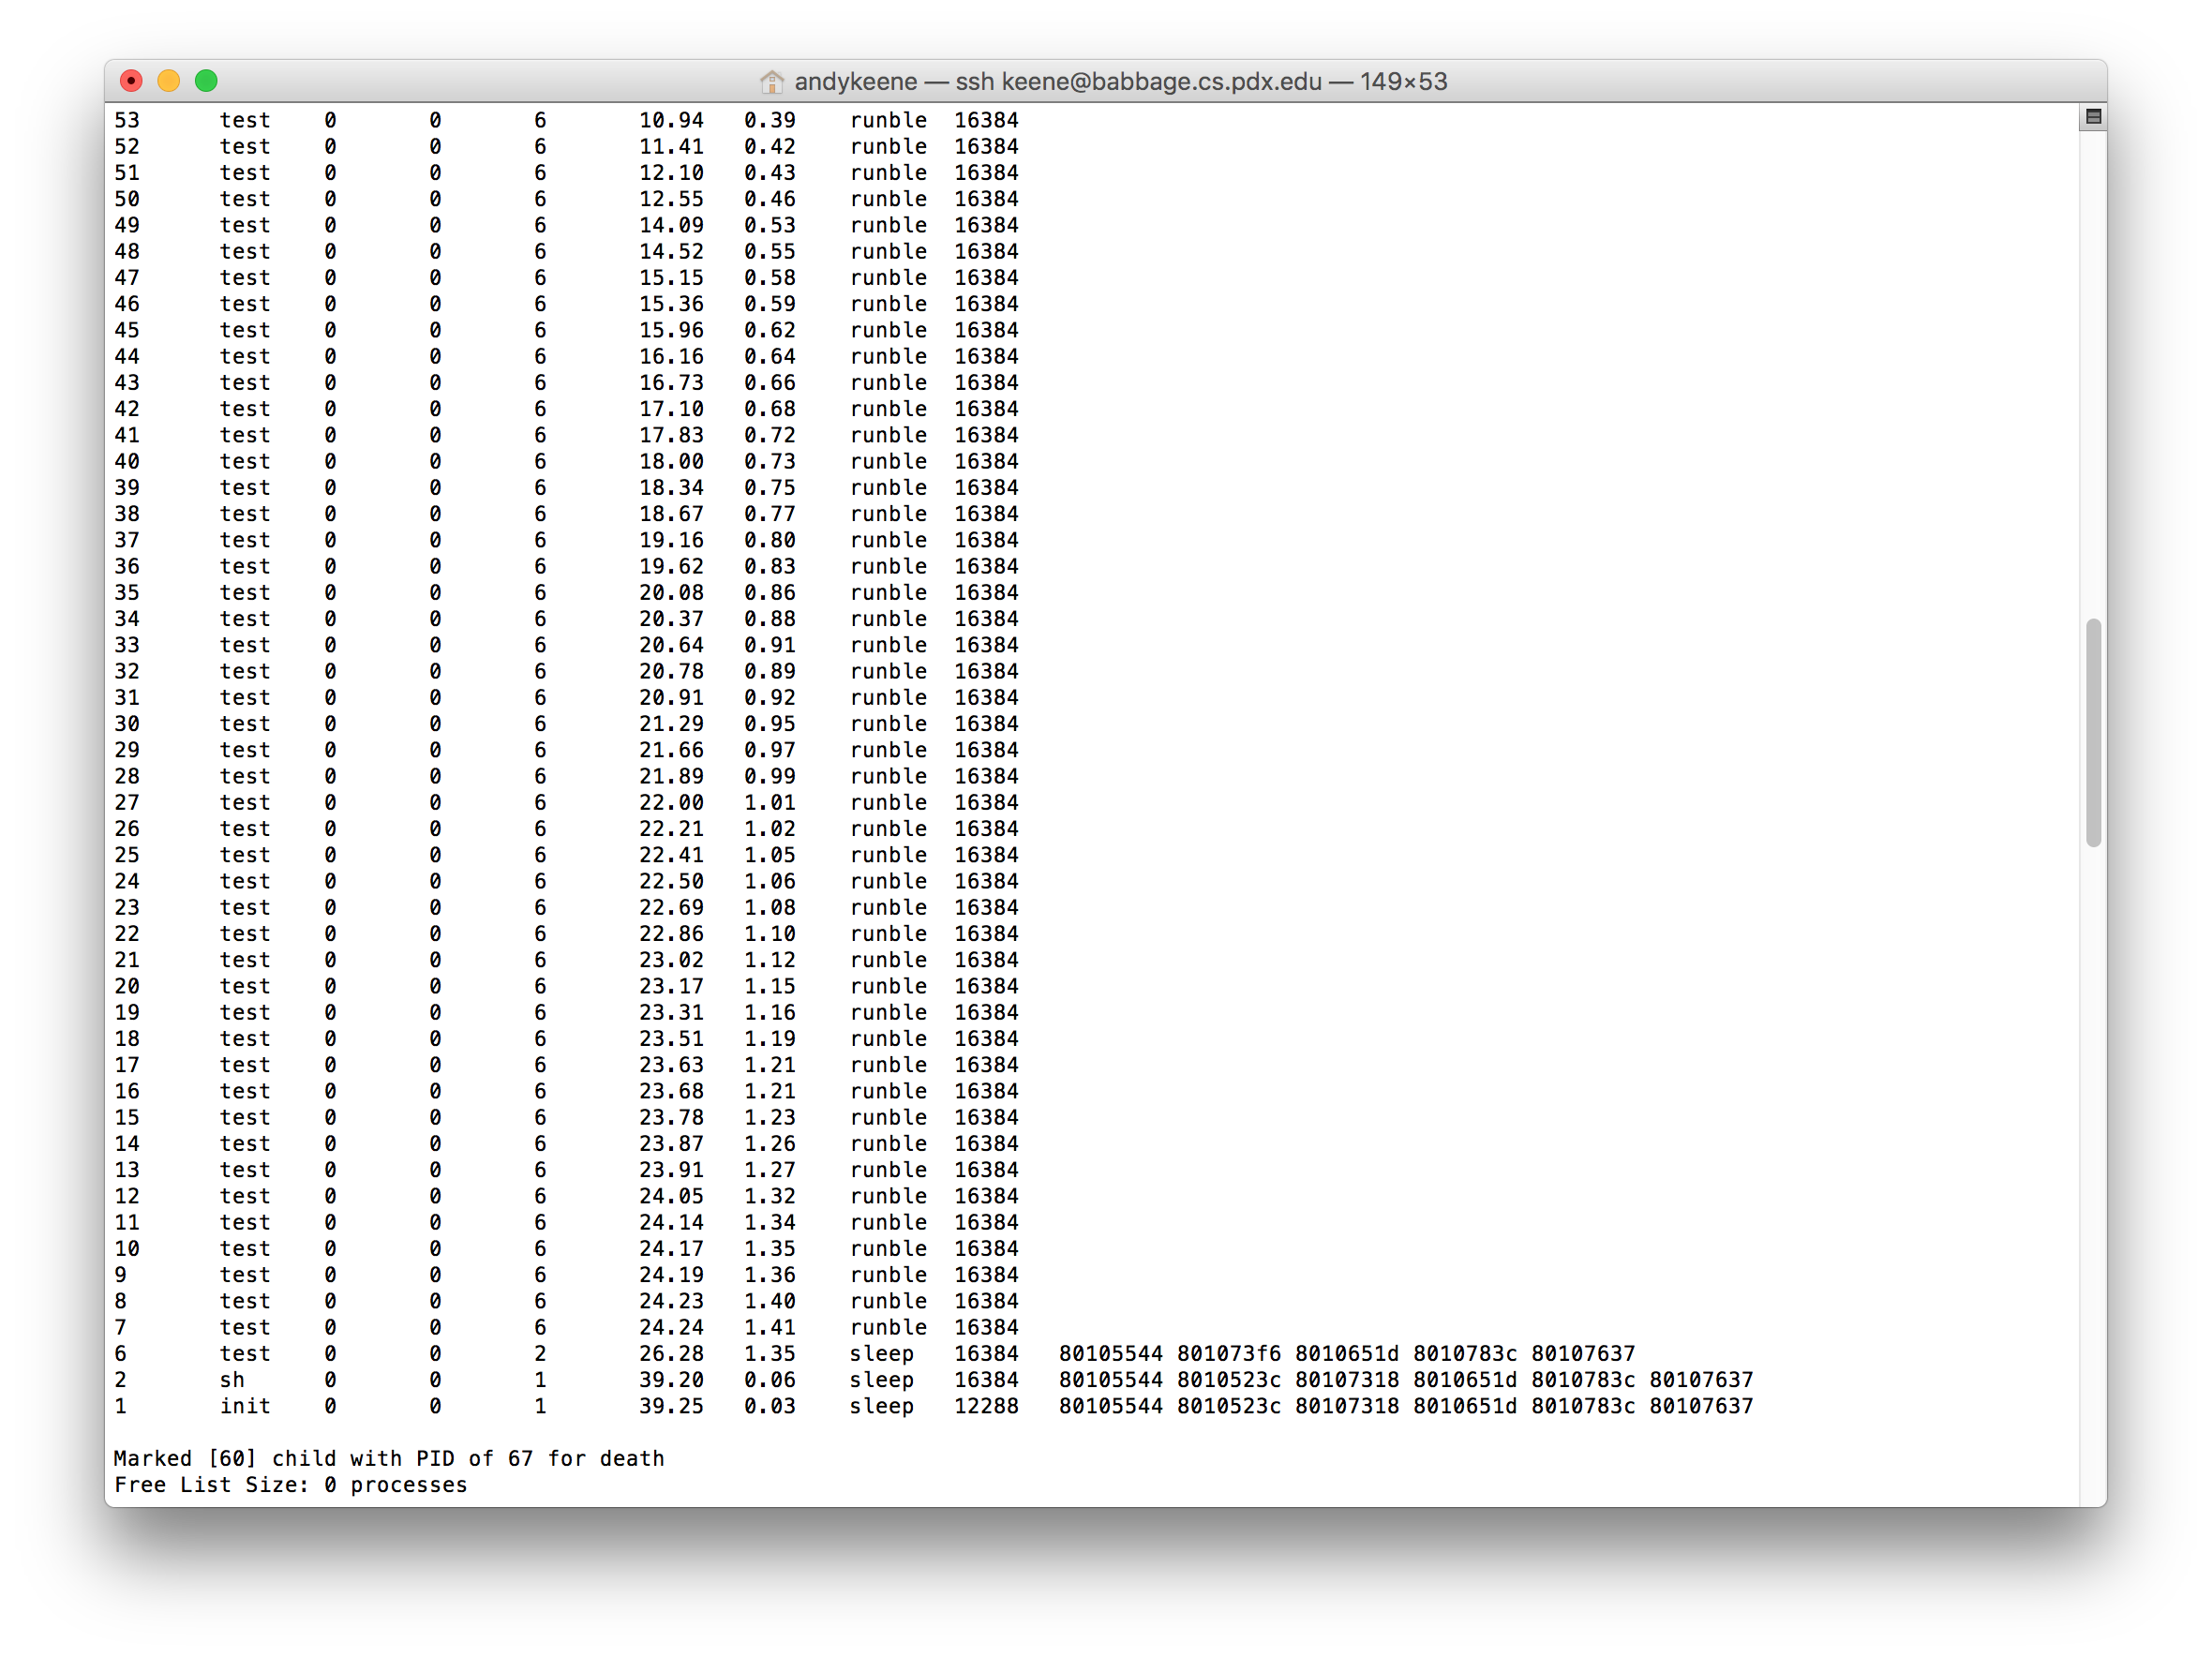
\includegraphics[width=0.8\linewidth]{zombie-processes.png}
\caption{more of ctrl-p output after forking}
\label{fig:3}
\end{figure}

\pagebreak
In figure 2, we see that parent created 61 children and has a PID of 6. In figures 3 and 4, using the output of \ctrl{p}, we see that the parent did in fact create 61 children (I'll let you count this one yourself); thus the number of process displayed by \ctrl{p} increased by the number of children, plus the parent, processes created. In total there are now $64$ active processes, which means since NPROC is 64, that there are no free processes left. \ctrl{f} is also seen in figure 2 displaying 0 processes on its list. This meets our expectations for this stage of the test, thus this step \textbf{PASSES}.

\pagebreak

\begin{figure}[h]
\centering
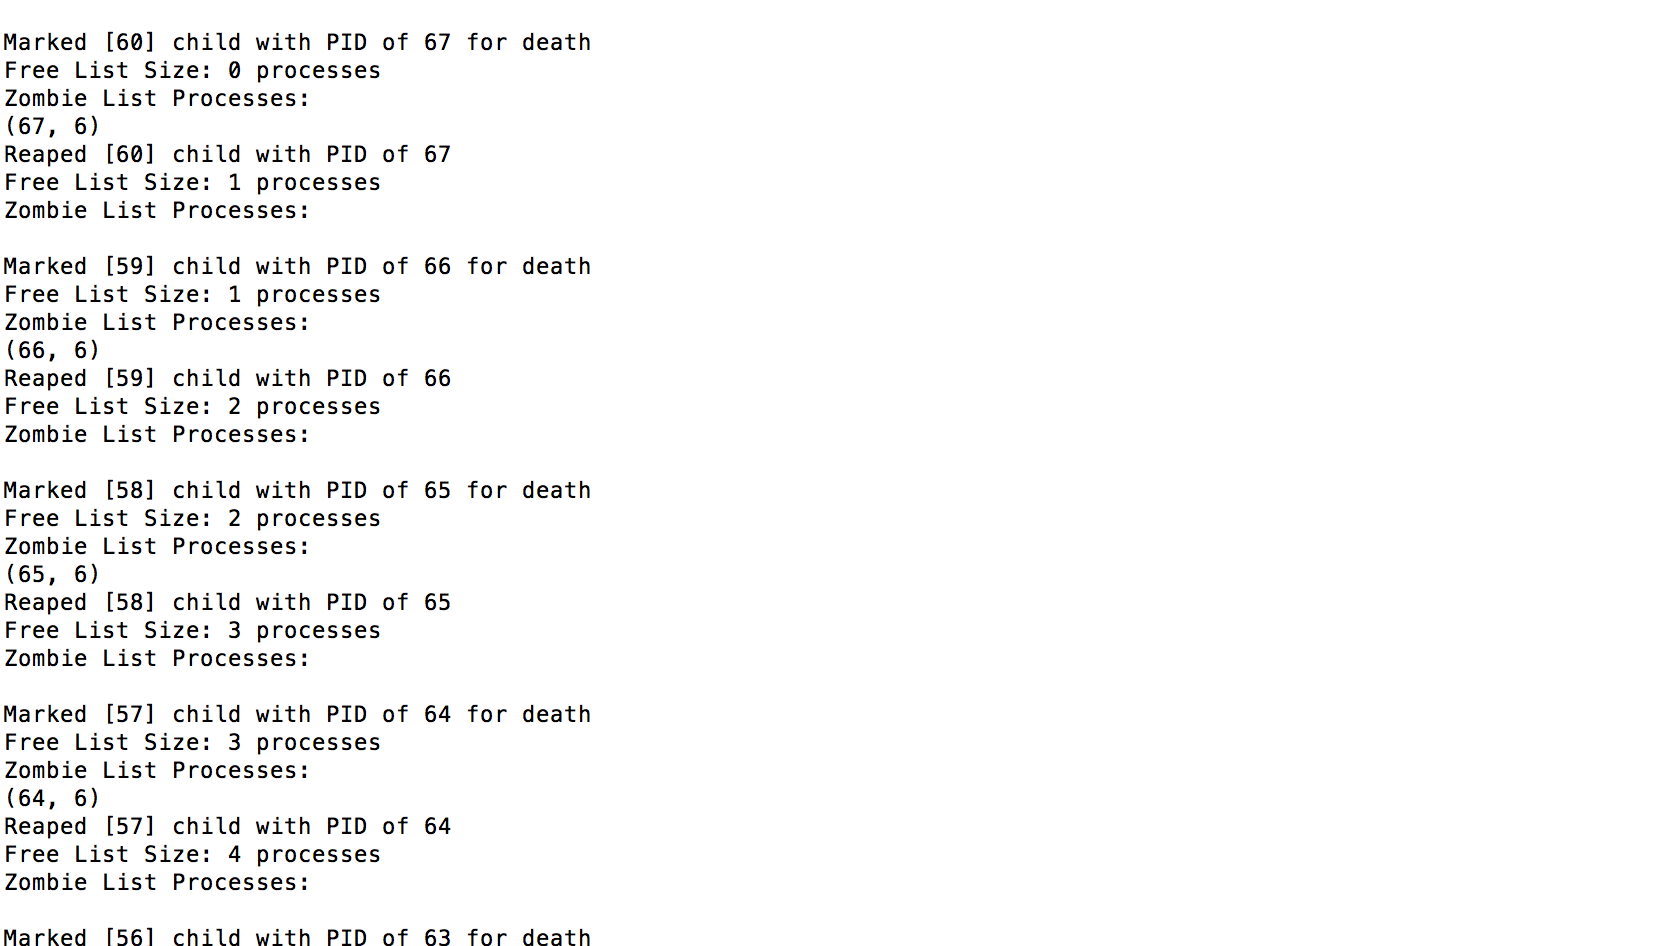
\includegraphics[width=0.8\linewidth]{zombie-during.png}
\caption{Reaping children}
\label{fig:4}
\end{figure}


Figure 4 shows the beginning of the reapings; we see that before that any child has been reaped that the size of the free list is still 0, that after a child has been marked it appears on the zombie list, \emph{and} that after the child is reaped (but before another one is killed) the zombie list becomes empty and the free list has increased by 1; this is also confirmed by the matching PID and PPID of the child and parent. Figure 5 shows more of this procedure. This meets our expectations for this stage of the test, thus this step \textbf{PASSES}.

\pagebreak


\begin{figure}[h]
\centering
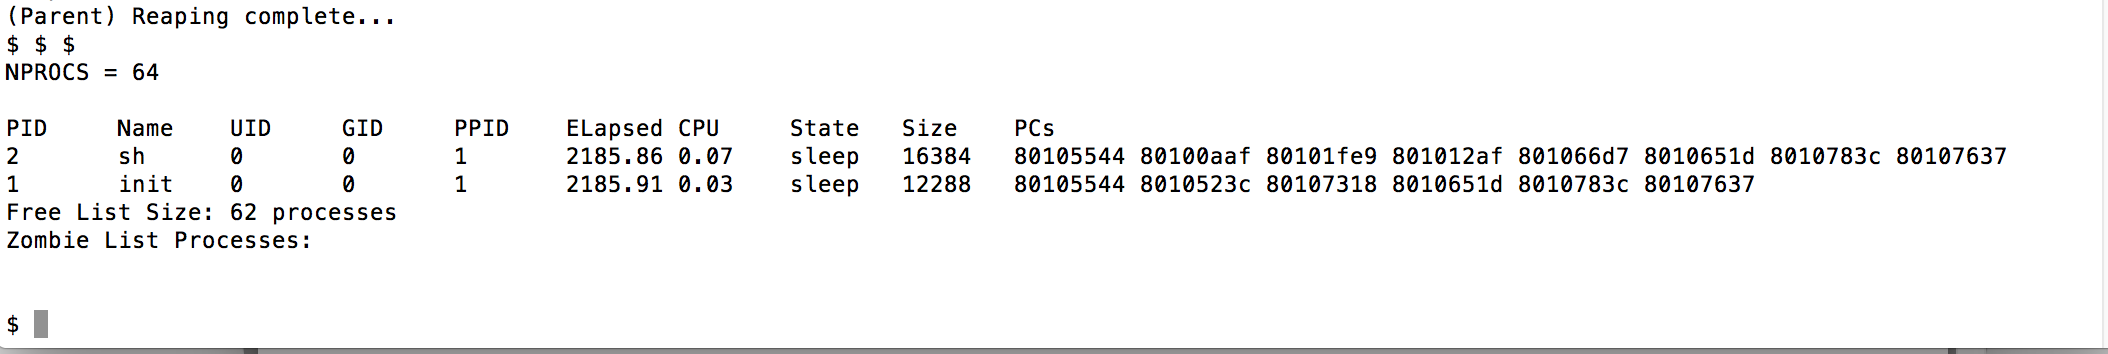
\includegraphics[width=0.8\linewidth]{zombie-after.png}
\caption{After parent exits}
\label{fig:5}
\end{figure}

For the final stage of this test, as seen in figure 6, the free list has returned to its initial size (again matching $|NPROCS| - active\  processes$) and that the zombie list is empty (matching \ctrl{p}). This meets our expectations for this stage of the test, thus this step \textbf{PASSES}.


Since at each step, or stage, of this step, this test \textbf{PASSES}; and further, because this test demonstrates requirements 1, 2, 6, 7.b, and 7.d we can conclude requirements 
1, 2, 6, 7.b, and 7.d are met.


\subsection*{Shell Kill Command (Requirement 3)}
For this test we will demonstrate requirement 3, that the shell {\tt kill} command correctly causes a process to transition to the ZOMBIE and UNUSED states accordingly. To this we will create an additional function {\tt inf\_loops()} in the user
{\tt test} program (test.c lines 153-165) that will fork 5 children where all of whom, including the parent, will spin indefinitely. The steps, and corresponding expectations of this test are laid out as follows:
	
	\begin{itemize}

		\item Before beginning we will verify the statuses of each list with \ctrl{p}, \ctrl{z}, and \ctrl{f} respectively. \ctrl{f} and \ctrl{z} were demonstrated to be correct in the test \emph{Free, \ctrl{f} and 
			Zombie, \ctrl{z}  (Requirements 1, 2, 6, 7.b, 7.d)}.
		\item We will invoke the {\tt test} program using the command {\tt \$ test \&} which will allow us to regain shell access in order to kill the created processes. We expect that the parent will display its PID. 
		\item Next, we will press \ctrl{p}, \ctrl{z}, and \ctrl{f} to see that the free list decreased by 6, that there are no zombie sinces all created processes are spinning, and that 6 additional 
			processes named \emph{test} now appear in the runnable/running state on \ctrl{p}.
		\item One by one we will kill the processes in descending order toward the parent. We must kill the parent last to enforce that the children are not automatically inherited by {\tt initproc}. We will press \ctrl{z} before
			and after killing each process. We expect the zombie list to grow by one between each {\tt kill} until the parent process is killed, and that format of the zombie list {\tt (PID, PPID)} will match the child just
			killed, and it's parent PID which was printed previously.
		\item Before killing the parent we will press \ctrl{f} and \ctrl{p}. Since the parent is still running, the children have not yet been reaped so we expect to see all 5 children on the zombie list (in reverse order of death),
			in the ZOMBIE state on \ctrl{p}, and that the free list \emph{has not} increased in size.
		\item We will finish by killing the parent. After killing the parent, we expect to see a printed line of "zombie!" for each child we killed, and the following output of \ctrl{z} to be empty; we also expect
			that after killing the parent  \ctrl{p} and \ctrl{f} will show that all the processes returned to the UNUSED list (implicitly by an increase in size of the free list and not shown as an \emph{active process}
			on \ctrl{p}).
			
	\end{itemize}

\pagebreak

\begin{figure}[h]
\centering
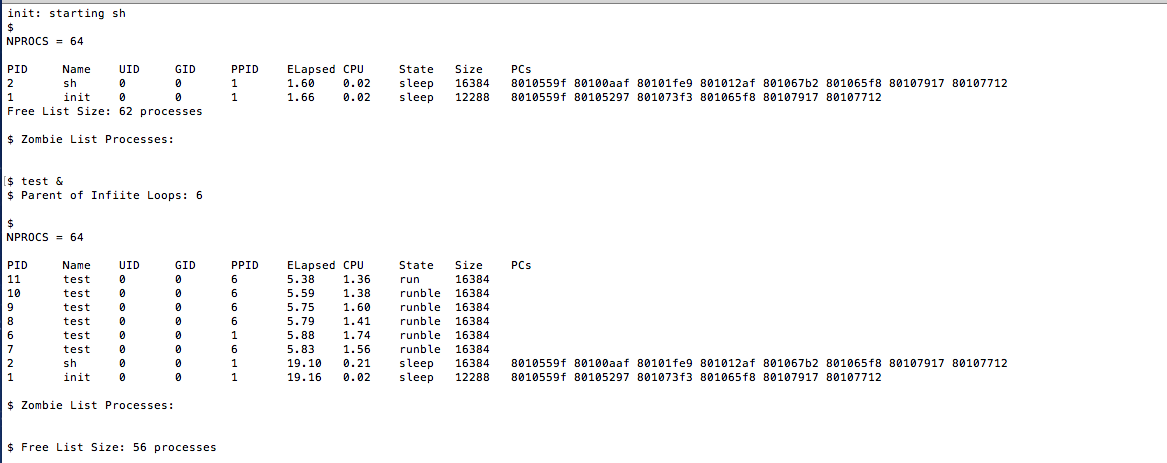
\includegraphics[width=0.8\linewidth]{shell-kill1.png}
\caption{Before and after spin start}
\label{fig:1}
\end{figure}

Here we see there are 62 free processes, that the parent has a PID of 6, and that after the spin tests are started through invoking {\tt test} that the free list decreased by 6, the correct amount, that the zombie list is empty and
that all children and the parent are in the runnable/running state. This meets our expectations for the first two stages.

\pagebreak


\begin{figure}[h]
\centering
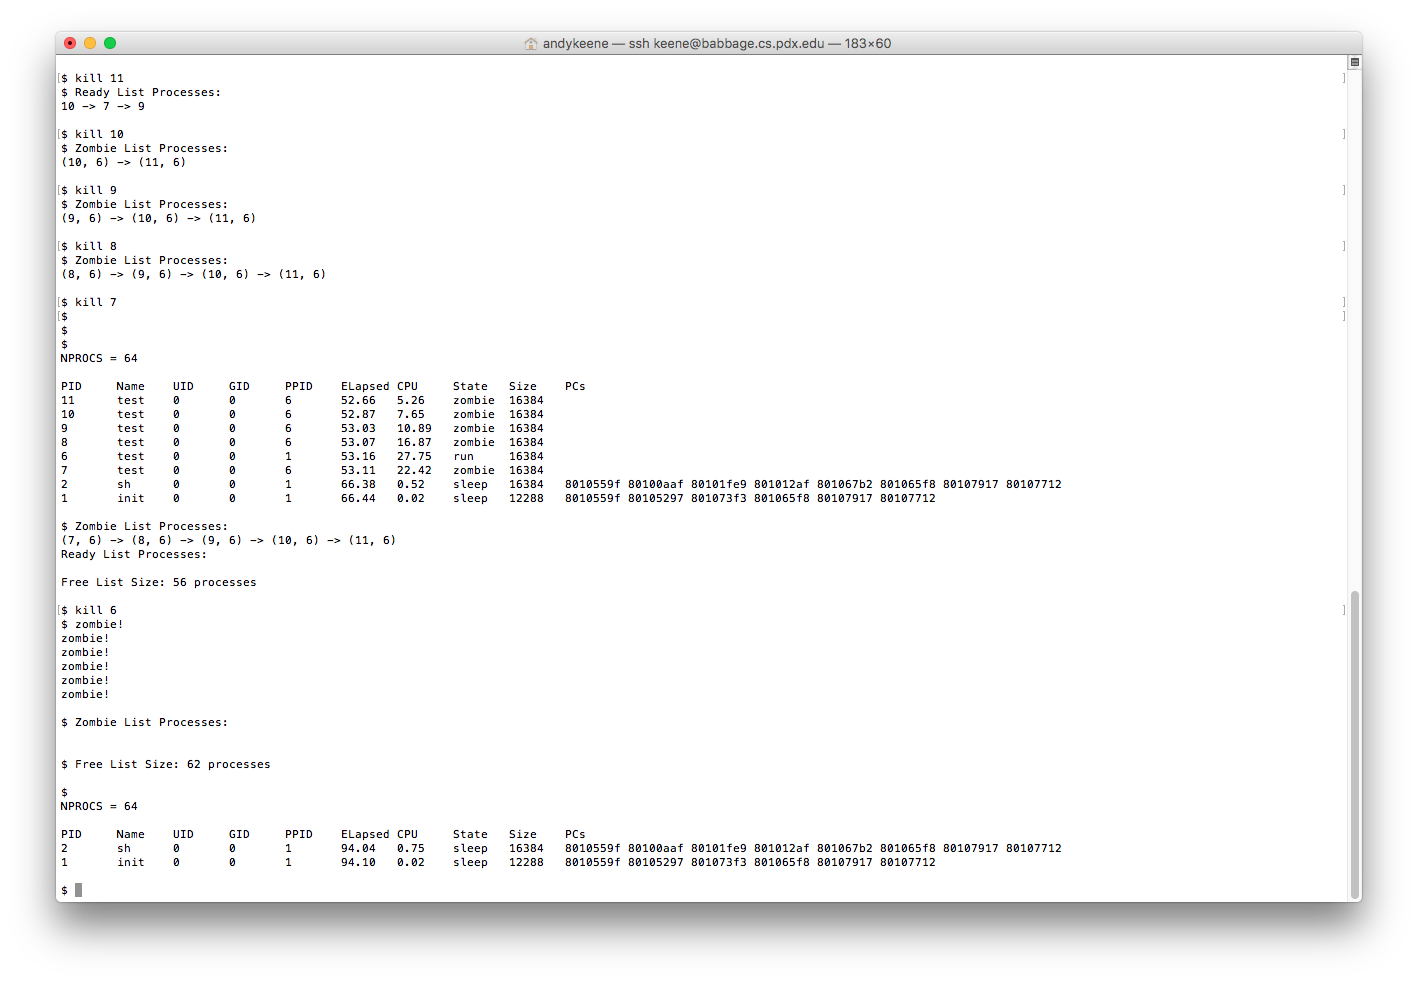
\includegraphics[width=0.8\linewidth]{shell-kill2.png}
\caption{Killing the children and parent}
\label{fig:2}
\end{figure}

Figure 2 shows that: the zombie list increasing by 1 with each child killed; that the order (in reverse order of being killed); before the parent is killed we see all of the children on the zombie list and all of them in the ZOMBIE state
on the \ctrl{p} output; and finally, that when the parent is killed the free list increases to its original size, the zombie list, and the ZOMBIE states in \ctrl{p} are all cleared.

Because our expectations for each stage of this test were met, this test \textbf{PASSES}.

\subsection*{Sleep, ctrl-s (Requirements 5, 7.c)}

This test will demonstrate that both the sleep list and ctrl-s function correctly:
	\begin{itemize}
		\item Before executing the user program {\tt test} we will will press ctrl-p and ctrl-s. This will be our baseline for the currently active processes before the test begins. Since the initial process is always sleeping on boot, 
			and {\tt sh} is waiting for input, we expect to find these on the list.
		\item Next the user program test will be called. Here, the function {\tt sleep\_test()} (test.c lines 145-151) will be called. The {\tt test} process will print its PID and then go to sleep for 5 seconds. Since the process must be running to print
			a message, we know it entered the SLEEPING state from RUNNING. After the message, we will press \ctrl{p} and \ctrl{s} again, expecting to find the process PID now in the SLEEPING sate, and
			on the sleeping list in addition to 
			{\tt init} and {\tt sh} ({\tt sh} is still waiting for our user program to exit). Note that we may have to press \ctrl{s} a few times since {\tt test} may be woken on interrupts, but put back to sleep because it is not time
			to wake up yet - inherent to the kernel.
		\item The process will notify us it is awake and exiting. We now expect it to be off of the sleeping list, and no longer in the output of \ctrl{p} since it exited; thus we expect \ctrl{p} and \ctrl{s} to return to their initial 
			outputs. 
	\end{itemize}


\begin{figure}[h]
\centering
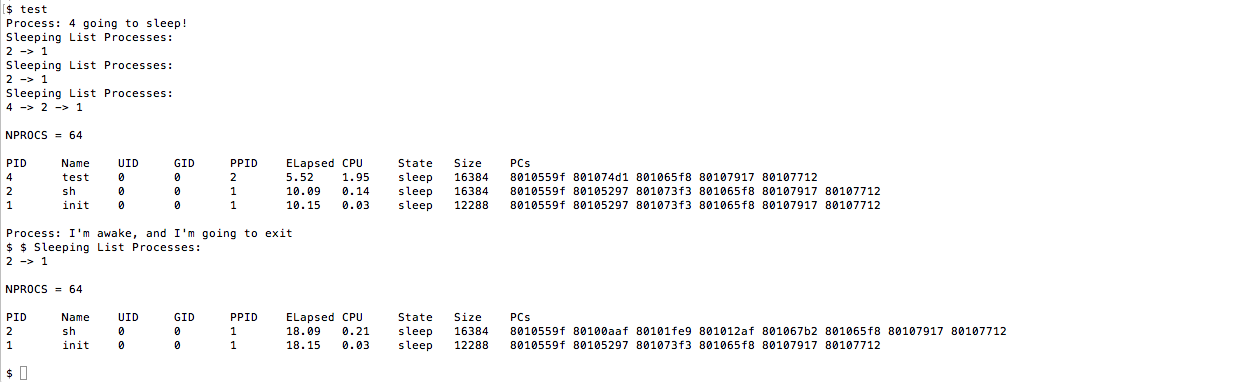
\includegraphics[width=0.8\linewidth]{sleep.png}
\caption{Sleep}
\label{fig:1}
\end{figure}

As we can see in figure 1: the initial output of \ctrl{p} and \ctrl{s} initially match with the expected processes on the list; next we can see that when {\tt test} goes to sleep that we did have to press \ctrl{s} multiple times
before finding it on the sleeping list but that the \ctrl{p} output asserts all processes on the list are in the correct state; and after {\tt test} exits, the sleeping list returns to it's initial state ({\tt sh} is waiting on input)
where {\tt test} is no longer to be found. Since all of our expectations were met, we have demonstrated that processes make the correct transitions from and to the SLEEPING state/list. Additionally, \ctrl{p} matches 
\ctrl{s} at each stage, demonstrating requirement 7.c. Thus, this test \textbf{PASSES}.

\subsection*{Round robin, ctrl-r (Requirements 4, 7.a)}
This test will demonstrate that processes scheduling enforces round robin, and that \ctrl{r} is working correctly. A function {\tt round\_robin()} will be added to the user program {\tt test} (text.c lines 172-184). This process will
create 20 children who will spin, along with the parent after the children's creation (21 total). We will then:

%Prior to the test we will establish that \ctrl{p} and \ctrl{r} match (no processes should be RUNNABLE/RUNNING at this time).  
	\begin{itemize}
		\item We will press \ctrl{p} and \ctrl{r} repeatedly to establish that \ctrl{r} does in fact display the ready list. Since two processes may be running at a time (two CPUs) and because context switches are far faster than we, 
			we must acknowledge a tolerant difference of \emph{at most} two processes between the outputs. The best way to assert this is that there must be at least 19 processes on the runnable list, and the output of \ctrl{p} 
			must have at least 19 {\tt test} processes in the RUNNABLE state, with the remaining in the RUNNING state (per list invariant they must be on one and only one).
		\item Next we will hold down \ctrl{r}. Again, with two CPUs, only 2 processes may be running at a time. Thus, from the 21 processes (children and parent), only two may be missing so we expect to see at least 19 on each output. 
		Additionally, we expect that since round robin is maintained that unless the scheduler has made it through the entire list, if some line is  A, D, E, J, H, K, P, Q, W and the next line starts with a K, then K must at least be 
		followed by P, Q, W (since K didn't run P, Q and W must not have either, thus the ordering remains) and P, Q, W must be followed by A, D, E and the two processes that \emph{were} running, in some order since these ran, and must be inserted into the back of the list.
	\end{itemize}
Asides: Some disorder in the rear of the list may occur between prints on \ctrl{r}. With two CPUs it may occur where one beats the other in placing a process back on the runnable list even though it was removed after the other. Thus disorder
may introduce itself by virtue of insertion order between the CPUs. This is why we are concerned with looked at the order of the middle of the list as outlined in the second stage of the test. It is also possible that ctrl-p or 
ctrl-r may obtain the lock in-between {\tt sched} and {\tt scheduler()} so that \emph{more} than 19 processes may be found in the RUNNABLE state which is why we focus on \emph{at least} 19.

\pagebreak

\begin{figure}[h]
\centering
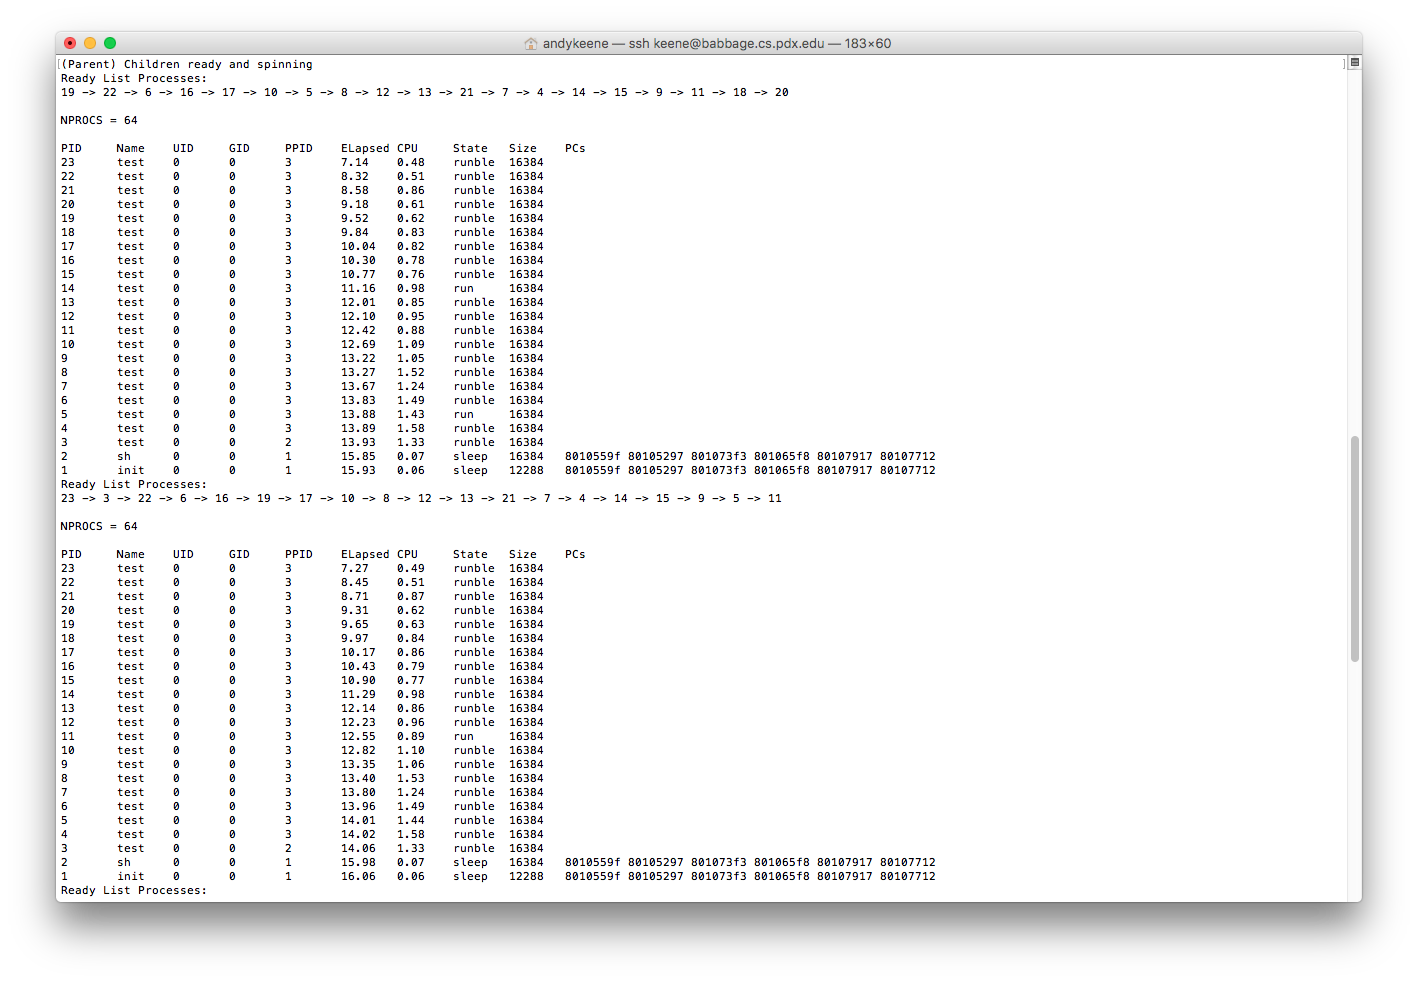
\includegraphics[width=0.8\linewidth]{rr-1.png}
\caption{ctrl-r and ctrl-p}
\label{fig:1}
\end{figure}  

\begin{figure}[h]
\centering
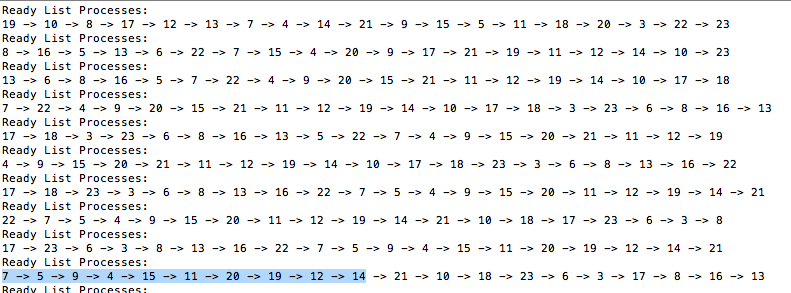
\includegraphics[width=0.8\linewidth]{rr-2.png}
\caption{round robin}
\label{fig:1}
\end{figure}

\pagebreak

In figure 1 we can see that there are in fact exactly 19 processes on the runnable list (all of which are {\tt test} PIDs, while on the output of \ctrl{p} there all of these PIDs are in the RUNNABLE or RUNNING state.

Each line on the runnable list never has less than 19 processes, all of the PIDs match those of the {\tt test} processes. If we take the front of each output of \ctrl{r} (head of the list) and find it on the list above we can see that
the ordering from it to the tail is maintained and after which we find elements that were ahead of it previously or not on the list (running). For example, on the highlighted line we find 7 (the head) on the line above and see from it to the end of the list is 
\emph{7, 5 , 9 , 4 , 15 , 11 , 20 , 19 , 12 , 14 , 21} - this exact order is maintained on the highlighted line with the elements previously ahead of 7 now at the end of the list! This matches our expectations.

Because \ctrl{r} and \ctrl{p} meet our expectations for the similarities we can prove, and because the round robin ordering described in the second stage was demonstrated we can conclude that this test \textbf{PASSES}. Thus
requirements 3 and 7.a are fulfilled.


As a resulting of all tests \textbf{PASSING} we can conclude that requirements 1-7 have been fulfilled. It should also be noted that the {\tt DEBUG} flag was turned on during testing, so before 
each addition and after each removal from a list, {\tt checkprocs()} verified, using the process table array, that each process was on one and only one list; additionally, the assertion by each helper
function that the lock is held when accessing a list helps to ensure atomicity of transitions. We believe this is sufficient supporting evidence that the mandatory invariant is held.
\end{document}




